\documentclass[a4paper,12pt]{exam}
	\usepackage{graphicx}
	\usepackage[utf8]{inputenc}
	\usepackage[T1]{fontenc}
	\usepackage{listings}
	\usepackage{color}
	\usepackage{amsmath}
	\usepackage{enumerate}
	\usepackage{caption}
	\usepackage{subcaption}


\begin{document}
\begingroup 
	  \bf \Large Mecânica Clássica I\\
	  \indent \normalsize André Del Bianco Giuffrida
	\endgroup
	\\ \quad
	\\
	Máquina de Atwood dupla
	\\ \\
	Inicialmente vamos definir os vínculos:\\
	Temos todas as massas vinculadas as cordas $l$, $l_1$ e $l_2$ \\
	Podemos definir a posição de cada uma das quatro massas ($m$, $2m$, $3m$ e $4m$) com base na posição de uma das duas polias suspensas;
	e da posição de uma massa em cada ramo, ou seja, precisamos de três coordenadas generalizadas.
	sendo assim vamos escrever a posição de cada uma das massas em função de $q$, $q_1$ e $q_2$ como mostra a figura.

	\begin{figure}[h]
		\centering
		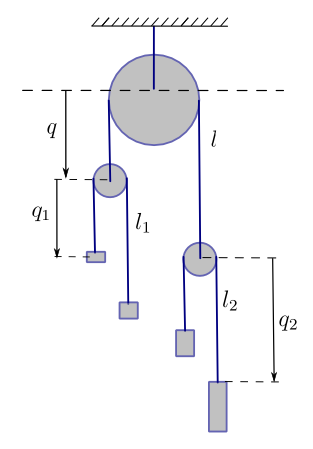
\includegraphics[scale=0.5]{Atwoood.png}
	\end{figure}
	
	de modo que se colocar-mos a referencia no centro da primeira polia podemos escrever:
	\[
	\begin{array}{ll}
	\text{para a massa } m_1 \text{:} & h_1 = q+q_1 \\
	\text{para a massa } m_2 \text{:} & h_2 = q+(l_1 - q_1) \\
	\text{para a massa } m_3 \text{:} & h_3 = (l-q)+(l_2-q_2) \\
	\text{para a massa } m_4 \text{:} & h_4 = (l-q)+q_2 \\ 
	\end{array}
	\]
	
	Podemos escrever assim as Energias do sistema:
	
	Para a Energia Potencial:
	\[ V = mg( -4q -q_1 + q_2 + 2l_1 + 3l_2 + 7l )\]
	
	Já para a Energia Cinética:
	
	\[ T = m \Big(\frac{(\dot{q}+\dot{q_1})^2}{2} + ( \dot{q}+\dot{l_1} - \dot{q_1})^2 + \frac{3(\dot{l}-\dot{q}+\dot{l_2}-\dot{q_2})^2}{2} + 2(\dot{l}- \dot{q}+\dot{q_2})^2 \Big) \]

	Usando o fato de que as cordas não esticam notamos que $\dot{l} = \dot{l_1} = \dot{l_2} = 0$
	
	\[ T = m \Big(\frac{(\dot{q}+\dot{q_1})^2}{2} + ( \dot{q}-\dot{q_1})^2 + \frac{3(-\dot{q}-\dot{q_2})^2}{2} + 2(-\dot{q}+\dot{q_2})^2 \Big) \]
	
	Calculando a Lagrangeana para o sistema temos
	
	\[ \mathcal{L} = T - V \]
	
	\[ \mathcal{L} = m\Bigg[ \frac{(\dot{q}+\dot{q_1})^2}{2} + (\dot{q}-\dot{q_1})^2 + \frac{3(-\dot{q}-\dot{q_2})^2}{2} + 2(-\dot{q}+\dot{q_2})^2 - g( -4q -q_1 + q_2 + 2l_1 + 3l_2 + 7l ) \Bigg] \]
	
	Pela Equação de Euler-Lagrange
	
	\[\frac{d}{dt} \frac{\partial \mathcal{L} }{\partial \dot{q_i}} - \frac{\partial \mathcal{L} }{\partial q_i }  = 0\]
	
	para $q$
	
	\[ \frac{\partial \mathcal{L} }{\partial \dot{q}} = m(\dot{q}+\dot{q_1} + 2\dot{q}-2\dot{q_1} + 3\dot{q} + 3\dot{q_2} +4\dot{q} - 4\dot{q_2}) = m(6\dot{q} -\dot{q_1} + 3\dot{q_2})\]
	
	\[ \frac{d}{dt} \frac{\partial \mathcal{L} }{\partial \dot{q}} = m(6\ddot{q} -\ddot{q_1} + 3\ddot{q_2})\]
	
	\[\frac{\partial \mathcal{L} }{\partial q } = 4mg, \quad \text{e assim ficamos com:} \quad (6\ddot{q} -\ddot{q_1} + 3\ddot{q_2}) = 4g\]
	
	para $q_1$
	
	\[\frac{\partial \mathcal{L} }{\partial \dot{q_1}} = m( \dot{q} + \dot{q_1} -2\dot{q} +2\dot{q_1} ) = m(-\dot{q}+3\dot{q_1} ) \quad \to \quad \frac{d}{dt}\frac{\partial \mathcal{L} }{\partial \dot{q_1}} = m(-\ddot{q}+3\ddot{q_1}) \]
	
	\[\frac{\partial \mathcal{L} }{\partial q_1} = mg, \quad \text{e assim ficamos com:} \quad (-\ddot{q}+3\ddot{q_1}) = g\]
	
	e para $q_2$
	
	\[ \frac{\partial \mathcal{L} }{\partial \dot{q_2}} = m(7\dot{q_2} -\dot{q}) \quad \to \quad \frac{d}{dt}\frac{\partial \mathcal{L} }{\partial \dot{q_2}} = m(7\ddot{q_2}-\ddot{q}) \]
	
	\[ \frac{\partial \mathcal{L} }{\partial q_2} = -mg, \quad \text{e assim ficamos com:} \quad (7\ddot{q_2}-\ddot{q}) = -g\]
	
	Com as três equações podemos resolver o problema.
	
	\[
	\begin{array}{rcl}
		(6\ddot{q} -\ddot{q_1} + 3\ddot{q_2}) & = & 4g \\
		(-\ddot{q}+3\ddot{q_1}) & = & g \\
		(-7\ddot{q_2}+\ddot{q}) & = & g \\
	\end{array}
	\]
	
	
	\[ \ddot{q} = \frac{25}{32}g \quad \quad \ddot{q_1} = \frac{19}{32}g \quad \quad \ddot{q_2} = -\frac{g}{32} \]		
		
	\begin{figure}[h]
		\centering
		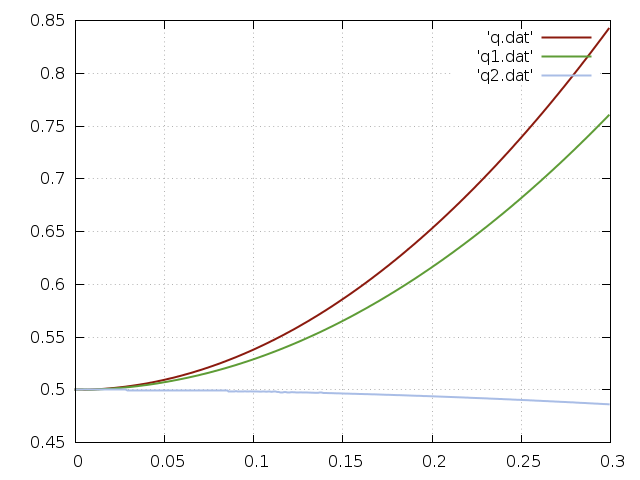
\includegraphics[scale=0.5]{Graph.png}
		\caption{Posição das coordenadas generalizadas por tempo}
	\end{figure}
	
	Usando a definição inicial das coordenadas escolhidas podemos saber as posições de cada uma das massas ($h_i$) em função do tempo. \\
	Partindo todas as massas da mesma altura $h_1 = h_2 = h_3 = h_4 = h$, podemos saber $q_{_{0}}$, $q_{1_0}$ e $q_{2_0}$.
	\[
	\begin{array}{ll}
	\text{para a massa } m_1 \text{:} & h = q_{_0} + q_{1_0} \\
	\text{para a massa } m_2 \text{:} & h = q_{_0} - q_{1_0} + l_1 \\
	\text{para a massa } m_3 \text{:} & h = l + l_2 - q_{_0} - q_{2_0} \\
	\text{para a massa } m_4 \text{:} & h = l - q_{_0} + q_{2_0} \\ 
	\end{array}
	\]
	
	\[h = \frac{1}{4}(2l +l_1 + l_2); \quad q_{_0} = \frac{1}{4} (2l-l_1+l_2); \quad q_{1_0} = \frac{l_1}{2}; \quad q_{2_0} = \frac{l_2}{2} \]
	
	\[
	\begin{array}{lclcccl}
	q(t) &=& q_{_0} + \frac{25}{64}gt^2 & = & \frac{1}{4} (2l-l_1+l_2) &+& \frac{25}{64}gt^2\\ \quad & \quad & \quad & \quad & \quad & \quad& \quad\\
	q_1(t) &=& q_{1_0} + \frac{19}{64}gt^2 & = & \frac{l_1}{2} &+& \frac{19}{64}gt^2\\ \quad & \quad & \quad & \quad & \quad & \quad& \quad\\
	q_2(t) &=& q_{2_0} - \frac{1}{64}gt^2 & = & \frac{l_2}{2} &-& \frac{1}{64}gt^2\\ \quad & \quad & \quad & \quad & \quad  & \quad& \quad\\
	
	\end{array}
	\]
	
	\begin{figure}[h]
		\centering
		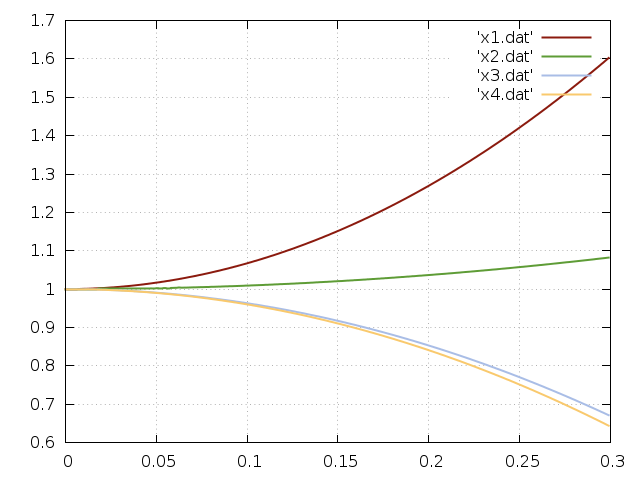
\includegraphics[scale=0.5]{Graph1.png}
		\caption{Posição das massas no tempo}
	\end{figure}
	Agora vamos achar as forças nos vínculos ou seja as trações nas cordas.
	e para isso vamos voltar na $\mathcal{L}$ porém vamos considerar  $\dot{l}$, $ \dot{l_1}$ e $\dot{l_2}$ ambas $\neq 0$ em $T$, com isso temos:
	\[ T = m \Big(\frac{(\dot{q}+\dot{q_1})^2}{2} + ( \dot{q}+\dot{l_1} - \dot{q_1})^2 + \frac{3(\dot{l}-\dot{q}+\dot{l_2}-\dot{q_2})^2}{2} + 2(\dot{l}- \dot{q}+\dot{q_2})^2 \Big) \]
	\[ V = mg( -4q -q_1 + q_2 + 2l_1 + 3l_2 + 7l )\]
	

	\[ \mathcal{L} = T - V \]
	
	\[ \mathcal{L} = m\Bigg[\Big(\frac{(\dot{q}+\dot{q_1})^2}{2} + ( \dot{q}+\dot{l_1} - \dot{q_1})^2 + \frac{3(\dot{l}-\dot{q}+\dot{l_2}-\dot{q_2})^2}{2} + 2(\dot{l}- \dot{q}+\dot{q_2})^2 \Big) - g( -4q -q_1 + q_2 + 2l_1 + 3l_2 + 7l ) \Bigg] \]
	
	sabemos pela equação de Euler-Lagreange que:
	
	\[ \frac{d}{dt}\frac{\partial \mathcal{L}}{\partial \dot{l_i}} -\frac{\partial \mathcal{L}}{\partial l_i} = T_i\]
	
	Para cada um dos vínculos, e assim podemos achar as Tensões $T_i$ nas cordas
	\\
	Para a corda $l$
	\[ m \Big[ 3(\ddot{l} -\ddot{q} + \ddot{l_2} - \ddot{q_2}) + 4(\ddot{l} - \ddot{q} + \ddot{q_2}) \Big]  +7mg = T \]
	Para a corda $l_1$
	\[ m\Big[ 2(\ddot{q} + \ddot{l_1} - \ddot{q_1}) \Big] +2mg = T_1\]
	Para a corda $l_2$
	\[ m\Big[ 3(\ddot{l} - \ddot{q} + \ddot{l_2} - \ddot{q_2}) \Big] + 3mg = T_2\]
	
	Aqui já sabemos $\ddot{q}$, $\ddot{q_1}$ e $\ddot{q_2}$ restando assim um sistema de três equações e três incógnitas, como segue:
	
	\[
		\begin{array}{rcl}
			3m\ddot{l} -3m\frac{25}{32}g + 3m\ddot{l_2} + 3m\frac{g}{32} + 4m\ddot{l} - 4m\frac{25}{32}g -4m\frac{g}{32} +7mg &=& T \\
			2m\frac{25}{32}g + 2m\ddot{l_1} - 2m\frac{19}{32}g + 2mg &=& T_1 \\
			3m\ddot{l} -3m\frac{25}{32}g + 3m\ddot{l_2} + 3m\frac{g}{32}+ 3mg &=& T_2 \\
		\end{array}
	\]
	
	\end{document}
